\documentclass[11pt,letterpaper]{article}

% =============================================================================
% PACKAGES
% =============================================================================
\usepackage[margin=1in]{geometry}
\usepackage{enumitem}
\usepackage{setspace}
\usepackage{graphicx}
\usepackage[table]{xcolor}
\usepackage{tikz}
\usetikzlibrary{shapes.geometric, arrows.meta, positioning, fit, backgrounds, calc, decorations.pathreplacing, trees, matrix, shapes.multipart, shapes.symbols}
\usepackage{tcolorbox}
\usepackage{booktabs}
\usepackage{longtable}
\usepackage{array}
\usepackage{tabularx}
\usepackage{multirow}
\usepackage{fancyhdr}
\usepackage{titlesec}
\usepackage[colorlinks=true,linkcolor=blue!60!black,urlcolor=blue!60!black,citecolor=blue!60!black]{hyperref}
\usepackage{bookmark}
\usepackage{parskip}
\usepackage{float}
\usepackage{caption}
\usepackage{subcaption}
\usepackage{listings}
\usepackage{microtype}
\usepackage{textcomp}
\usepackage{amssymb}
\usepackage{pifont}

% =============================================================================
% CONFIGURATION
% =============================================================================
\setstretch{1.15}

% Define colors
\definecolor{primary}{RGB}{50, 90, 50}
\definecolor{secondary}{RGB}{80, 130, 80}
\definecolor{accent}{RGB}{180, 70, 50}
\definecolor{success}{RGB}{40, 150, 80}
\definecolor{warning}{RGB}{220, 160, 40}
\definecolor{critical}{RGB}{200, 60, 60}
\definecolor{lightgray}{RGB}{245, 245, 245}
\definecolor{darkgray}{RGB}{80, 80, 80}
\definecolor{monitorcolor}{RGB}{220, 240, 255}
\definecolor{alertcolor}{RGB}{255, 235, 220}
\definecolor{processcolor}{RGB}{230, 255, 230}
\definecolor{toolcolor}{RGB}{240, 235, 255}
\definecolor{metriccolor}{RGB}{255, 250, 220}
\definecolor{incidentcolor}{RGB}{255, 230, 230}

% Section formatting
\titleformat{\section}{\Large\bfseries\color{primary}}{\thesection}{1em}{}[\titlerule]
\titleformat{\subsection}{\large\bfseries\color{secondary}}{\thesubsection}{1em}{}
\titleformat{\subsubsection}{\normalsize\bfseries\color{darkgray}}{\thesubsubsection}{1em}{}

% Header/Footer
\pagestyle{fancy}
\fancyhf{}
\fancyhead[L]{\small\textcolor{darkgray}{Operational Viewpoint Specification}}
\fancyhead[R]{\small\textcolor{darkgray}{Architecture Documentation}}
\fancyfoot[C]{\thepage}
\renewcommand{\headrulewidth}{0.4pt}

% Custom environments
\newtcolorbox{definitionbox}[1][]{
    colback=lightgray,
    colframe=primary,
    fonttitle=\bfseries,
    title={#1},
    boxrule=0.5pt,
    arc=2pt,
    left=8pt,
    right=8pt,
    top=6pt,
    bottom=6pt
}

\newtcolorbox{examplebox}[1][]{
    colback=white,
    colframe=secondary,
    fonttitle=\bfseries,
    title={#1},
    boxrule=0.5pt,
    arc=2pt,
    left=8pt,
    right=8pt,
    top=6pt,
    bottom=6pt
}

\newtcolorbox{warningbox}[1][]{
    colback=orange!5,
    colframe=accent,
    fonttitle=\bfseries,
    title={#1},
    boxrule=0.5pt,
    arc=2pt,
    left=8pt,
    right=8pt,
    top=6pt,
    bottom=6pt
}

\newtcolorbox{guidancebox}[1][]{
    colback=green!5,
    colframe=success,
    fonttitle=\bfseries,
    title={#1},
    boxrule=0.5pt,
    arc=2pt,
    left=8pt,
    right=8pt,
    top=6pt,
    bottom=6pt
}

\newtcolorbox{patternbox}[1][]{
    colback=blue!3,
    colframe=primary!70,
    fonttitle=\bfseries,
    title={#1},
    boxrule=0.5pt,
    arc=2pt,
    left=8pt,
    right=8pt,
    top=6pt,
    bottom=6pt
}

\newtcolorbox{criticalbox}[1][]{
    colback=red!5,
    colframe=critical,
    fonttitle=\bfseries,
    title={#1},
    boxrule=0.5pt,
    arc=2pt,
    left=8pt,
    right=8pt,
    top=6pt,
    bottom=6pt
}

\newtcolorbox{slobox}[1][]{
    colback=yellow!5,
    colframe=warning,
    fonttitle=\bfseries,
    title={#1},
    boxrule=0.5pt,
    arc=2pt,
    left=8pt,
    right=8pt,
    top=6pt,
    bottom=6pt
}

% Listings configuration
\lstset{
    basicstyle=\ttfamily\small,
    backgroundcolor=\color{lightgray},
    frame=single,
    framerule=0.5pt,
    rulecolor=\color{darkgray},
    breaklines=true,
    captionpos=b,
    tabsize=2,
    showstringspaces=false,
    numbers=left,
    numberstyle=\tiny\color{darkgray},
    numbersep=5pt,
    xleftmargin=15pt
}

\lstdefinelanguage{yaml}{
    keywords={true,false,null,y,n},
    sensitive=false,
    comment=[l]{\#},
    morecomment=[s]{/*}{*/},
    morestring=[b]',
    morestring=[b]"
}

% Table column types
\newcolumntype{L}[1]{>{\raggedright\arraybackslash}p{#1}}
\newcolumntype{C}[1]{>{\centering\arraybackslash}p{#1}}
\newcolumntype{R}[1]{>{\raggedleft\arraybackslash}p{#1}}

% Custom commands
\newcommand{\cmark}{\ding{51}}
\newcommand{\xmark}{\ding{55}}

% =============================================================================
% DOCUMENT BEGIN
% =============================================================================
\begin{document}

% -----------------------------------------------------------------------------
% TITLE PAGE
% -----------------------------------------------------------------------------
\hypersetup{pageanchor=false}
\begin{titlepage}
    \centering
    \vspace*{1.5cm}
    
    {\Huge\bfseries\color{primary} Operational Viewpoint\par}
    \vspace{0.5cm}
    {\Large\color{secondary} Architecture Viewpoint Specification\par}
    \vspace{0.3cm}
    {\large\color{darkgray} System Operations, Monitoring \& Administration\par}
    
    \vspace{1.3cm}
    
    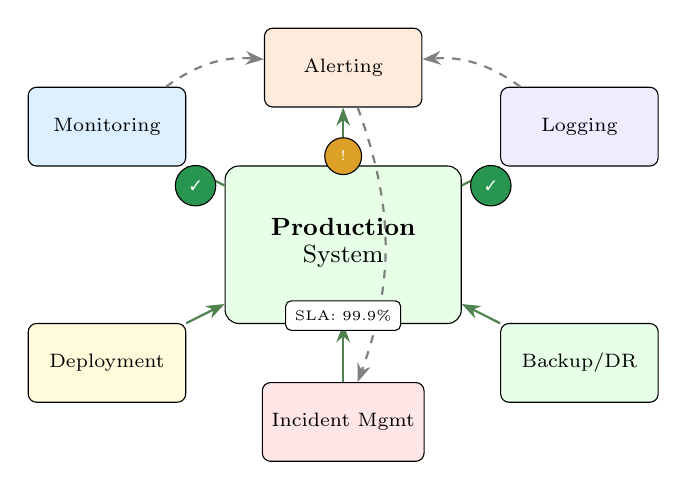
\begin{tikzpicture}[scale=0.75]
        % Central system
        \node[draw, rounded corners=5pt, fill=processcolor, minimum width=3cm, minimum height=2cm] (system) at (0, 0) {};
        \node[font=\small\bfseries] at (0, 0.3) {Production};
        \node[font=\small] at (0, -0.2) {System};
        
        % Monitoring
        \node[draw, rounded corners=3pt, fill=monitorcolor, minimum width=2cm, minimum height=1cm, font=\scriptsize] (monitor) at (-4, 2) {Monitoring};
        \node[draw, rounded corners=3pt, fill=alertcolor, minimum width=2cm, minimum height=1cm, font=\scriptsize] (alert) at (0, 3) {Alerting};
        \node[draw, rounded corners=3pt, fill=toolcolor, minimum width=2cm, minimum height=1cm, font=\scriptsize] (logging) at (4, 2) {Logging};
        
        % Operations
        \node[draw, rounded corners=3pt, fill=metriccolor, minimum width=2cm, minimum height=1cm, font=\scriptsize] (deploy) at (-4, -2) {Deployment};
        \node[draw, rounded corners=3pt, fill=incidentcolor, minimum width=2cm, minimum height=1cm, font=\scriptsize] (incident) at (0, -3) {Incident Mgmt};
        \node[draw, rounded corners=3pt, fill=processcolor, minimum width=2cm, minimum height=1cm, font=\scriptsize] (backup) at (4, -2) {Backup/DR};
        
        % Connections
        \draw[-{Stealth}, thick, secondary] (system) -- (monitor);
        \draw[-{Stealth}, thick, secondary] (system) -- (alert);
        \draw[-{Stealth}, thick, secondary] (system) -- (logging);
        \draw[-{Stealth}, thick, secondary] (deploy) -- (system);
        \draw[-{Stealth}, thick, secondary] (incident) -- (system);
        \draw[-{Stealth}, thick, secondary] (backup) -- (system);
        
        % Circular flow indicators
        \draw[-{Stealth}, thick, dashed, gray] (monitor) to[bend left=20] (alert);
        \draw[-{Stealth}, thick, dashed, gray] (alert) to[bend left=20] (incident);
        \draw[-{Stealth}, thick, dashed, gray] (logging) to[bend right=20] (alert);
        
        % Metrics indicators
        \node[draw, circle, fill=success, minimum size=0.4cm, font=\tiny, text=white] at (-2.5, 1) {\cmark};
        \node[draw, circle, fill=warning, minimum size=0.4cm, font=\tiny, text=white] at (0, 1.5) {!};
        \node[draw, circle, fill=success, minimum size=0.4cm, font=\tiny, text=white] at (2.5, 1) {\cmark};
        
        % SLA indicator
        \node[draw, rounded corners=2pt, fill=white, font=\tiny] at (0, -1.2) {SLA: 99.9\%};
    \end{tikzpicture}
    
    \vspace{1.5cm}
    
    \begin{tabular}{ll}
        \textbf{Version:} & 2.0 \\
        \textbf{Status:} & Release \\
        \textbf{Classification:} & ISO/IEC/IEEE 42010 Compliant \\
        \textbf{Last Updated:} & \today \\
    \end{tabular}
    
    \vfill
    
    {\small Based on the Views and Beyond approach to software architecture documentation}
    
\end{titlepage}
\hypersetup{pageanchor=true}
\setcounter{page}{1}

% -----------------------------------------------------------------------------
% TABLE OF CONTENTS
% -----------------------------------------------------------------------------
\tableofcontents
\newpage

% =============================================================================
% SECTION: VIEWPOINT NAME
% =============================================================================
\section{Viewpoint Name}

\begin{definitionbox}[Viewpoint Identification]
\begin{tabular}{@{}L{3.5cm}L{10cm}@{}}
\textbf{Name:} & Operational Viewpoint \\[0.5em]
\textbf{Synonyms:} & Operations View, Production View, Administration Viewpoint, System Management View, Runtime Operations View, Site Reliability View, Platform Operations View \\[0.5em]
\textbf{Identifier:} & VP-OPS-001 \\[0.5em]
\textbf{Version:} & 2.0 \\
\end{tabular}
\end{definitionbox}

\subsection{Viewpoint Classification}

The Operational Viewpoint addresses how a system is operated, administered, monitored, and maintained in production environments. While the Views and Beyond approach does not explicitly define an operational viewpoint as a primary style, operational concerns are critical cross-cutting aspects that intersect with deployment, component-and-connector, and quality attribute perspectives. This viewpoint provides essential guidance for running systems reliably in production.

\begin{table}[H]
\centering
\caption{Viewpoint Classification Taxonomy}
\begin{tabular}{@{}L{4cm}L{10cm}@{}}
\toprule
\textbf{Attribute} & \textbf{Value} \\
\midrule
Style Family & Cross-Cutting / Quality-Focused \\
Primary Focus & Production Operations and System Management \\
Abstraction Level & Operational / Runtime \\
Temporal Perspective & Runtime and Ongoing Operations \\
Related Styles & Deployment, C\&C, Service-Oriented \\
IEEE 42010 Category & Operational Viewpoint \\
Industry Alignment & Site Reliability Engineering (SRE), DevOps, ITIL \\
\bottomrule
\end{tabular}
\end{table}

\subsection{Viewpoint Scope}

The Operational Viewpoint encompasses multiple aspects of system operations:

\begin{itemize}
    \item \textbf{Observability:} Monitoring, logging, tracing, and metrics collection to understand system behavior and health in production.
    
    \item \textbf{Alerting and Incident Management:} Detection of anomalies, alert routing, incident response procedures, and escalation paths.
    
    \item \textbf{Deployment and Release:} Procedures for deploying, updating, and rolling back system changes safely.
    
    \item \textbf{Scaling and Capacity:} Mechanisms for handling load variations, capacity planning, and resource management.
    
    \item \textbf{Backup and Recovery:} Data protection, disaster recovery procedures, and business continuity planning.
    
    \item \textbf{Maintenance and Administration:} Routine operational tasks, configuration management, and system administration.
    
    \item \textbf{Service Level Management:} SLAs, SLOs, SLIs, error budgets, and service quality tracking.
    
    \item \textbf{Security Operations:} Runtime security monitoring, vulnerability management, and incident response.
\end{itemize}

% =============================================================================
% SECTION: OVERVIEW
% =============================================================================
\section{Overview}

The Operational Viewpoint provides a comprehensive framework for documenting how a software system is operated, monitored, and maintained throughout its production lifecycle. In modern systems where availability and reliability are critical, this viewpoint is essential for ensuring systems meet their service level commitments.

\subsection{Purpose and Scope}

The primary purpose of this viewpoint is to establish a clear understanding of operational requirements, procedures, and mechanisms that enable reliable system operation. This includes defining what needs to be monitored, how problems are detected and resolved, how changes are deployed safely, and how the system recovers from failures.

\begin{definitionbox}[Viewpoint Definition]
The Operational Viewpoint defines the mechanisms, procedures, and organizational structures required to operate a system in production. It encompasses observability infrastructure, incident management processes, deployment procedures, capacity management, disaster recovery capabilities, and service level definitions. This viewpoint bridges development activities with production operations.
\end{definitionbox}

\subsection{Key Characteristics}

The Operational Viewpoint exhibits several distinctive characteristics:

\textbf{Production Focus:} This viewpoint is concerned exclusively with the system in production environments, addressing the realities of operating software at scale with real users and data.

\textbf{Process and Procedure Emphasis:} Beyond technical mechanisms, this viewpoint documents the human processes, runbooks, and procedures essential for effective operations.

\textbf{Continuous Improvement:} Operations is iterative; this viewpoint supports ongoing refinement based on incidents, metrics, and changing requirements.

\textbf{Cross-Functional Integration:} Effective operations require coordination between development, operations, security, and business teams. This viewpoint facilitates that integration.

\textbf{Measurability:} Operational concerns are quantified through metrics, SLOs, and SLAs, enabling objective assessment of operational effectiveness.

\subsection{Relationship to Other Viewpoints}

The Operational Viewpoint connects to other architectural viewpoints in critical ways:

\begin{table}[H]
\centering
\caption{Relationships to Other Viewpoints}
\begin{tabular}{@{}L{3.5cm}L{10.5cm}@{}}
\toprule
\textbf{Viewpoint} & \textbf{Relationship} \\
\midrule
Deployment & Deployment topology defines what is operated. Infrastructure choices affect operational capabilities. \\
\addlinespace
Component-and-Connector & Runtime components are the units of monitoring. Connector protocols affect observability options. \\
\addlinespace
Information/Data & Data stores require backup and recovery. Data flows affect monitoring points. \\
\addlinespace
Development & Module structure affects deployment units. Build outputs become operational artifacts. \\
\addlinespace
Security & Security monitoring integrates with operational monitoring. Incident response covers security incidents. \\
\addlinespace
Quality Attribute & Availability, performance, and reliability requirements drive operational mechanisms. \\
\bottomrule
\end{tabular}
\end{table}

\subsection{Operational Architecture Overview}

\begin{figure}[H]
\centering
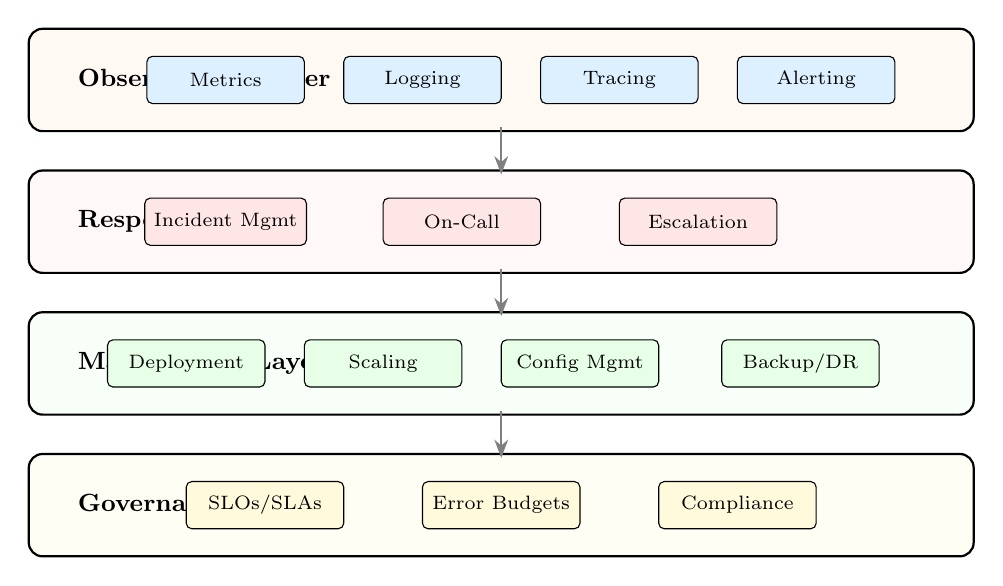
\begin{tikzpicture}[
    node distance=1.2cm and 1.5cm,
    layer/.style={draw, thick, rounded corners=5pt, minimum width=12cm, minimum height=1.3cm, font=\small},
    component/.style={draw, fill=monitorcolor, rounded corners=2pt, minimum width=2cm, minimum height=0.6cm, font=\scriptsize},
    arrow/.style={-{Stealth}, thick, gray}
]
    % Layers
    \node[layer, fill=alertcolor!30] (observe) at (0, 4) {};
    \node[font=\small\bfseries, anchor=west] at (-5.5, 4) {Observability Layer};
    
    \node[layer, fill=incidentcolor!30] (respond) at (0, 2.2) {};
    \node[font=\small\bfseries, anchor=west] at (-5.5, 2.2) {Response Layer};
    
    \node[layer, fill=processcolor!30] (manage) at (0, 0.4) {};
    \node[font=\small\bfseries, anchor=west] at (-5.5, 0.4) {Management Layer};
    
    \node[layer, fill=metriccolor!30] (govern) at (0, -1.4) {};
    \node[font=\small\bfseries, anchor=west] at (-5.5, -1.4) {Governance Layer};
    
    % Observability components
    \node[component] at (-3.5, 4) {Metrics};
    \node[component] at (-1, 4) {Logging};
    \node[component] at (1.5, 4) {Tracing};
    \node[component] at (4, 4) {Alerting};
    
    % Response components
    \node[component, fill=incidentcolor] at (-3.5, 2.2) {Incident Mgmt};
    \node[component, fill=incidentcolor] at (-0.5, 2.2) {On-Call};
    \node[component, fill=incidentcolor] at (2.5, 2.2) {Escalation};
    
    % Management components
    \node[component, fill=processcolor] at (-4, 0.4) {Deployment};
    \node[component, fill=processcolor] at (-1.5, 0.4) {Scaling};
    \node[component, fill=processcolor] at (1, 0.4) {Config Mgmt};
    \node[component, fill=processcolor] at (3.8, 0.4) {Backup/DR};
    
    % Governance components
    \node[component, fill=metriccolor] at (-3, -1.4) {SLOs/SLAs};
    \node[component, fill=metriccolor] at (0, -1.4) {Error Budgets};
    \node[component, fill=metriccolor] at (3, -1.4) {Compliance};
    
    % Arrows between layers
    \draw[arrow] (0, 3.4) -- (0, 2.8);
    \draw[arrow] (0, 1.6) -- (0, 1);
    \draw[arrow] (0, -0.2) -- (0, -0.8);
    
\end{tikzpicture}
\caption{Operational Architecture Layers}
\end{figure}

% =============================================================================
% SECTION: CONCERNS
% =============================================================================
\section{Concerns}

This section enumerates the architectural concerns that the Operational Viewpoint is designed to address. These concerns represent the fundamental questions stakeholders have about system operations.

\subsection{Primary Concerns}

\begin{enumerate}[label=\textbf{C\arabic*:}, leftmargin=2.5em]
    \item \textbf{System Observability}
    \begin{itemize}[nosep]
        \item What metrics indicate system health and performance?
        \item How are logs collected, aggregated, and searched?
        \item How are distributed requests traced across services?
        \item What dashboards provide operational visibility?
        \item How is observability data retained and accessed?
    \end{itemize}
    
    \item \textbf{Alerting and Notification}
    \begin{itemize}[nosep]
        \item What conditions trigger alerts?
        \item How are alerts routed to appropriate responders?
        \item What severity levels and escalation paths exist?
        \item How is alert fatigue minimized?
        \item What notification channels are used?
    \end{itemize}
    
    \item \textbf{Incident Management}
    \begin{itemize}[nosep]
        \item How are incidents detected, classified, and tracked?
        \item What is the incident response process?
        \item How are on-call rotations managed?
        \item What escalation procedures exist?
        \item How are post-incident reviews conducted?
    \end{itemize}
    
    \item \textbf{Deployment and Release}
    \begin{itemize}[nosep]
        \item How are changes deployed to production?
        \item What deployment strategies are used (blue-green, canary, rolling)?
        \item How are rollbacks performed?
        \item What approval and change management processes exist?
        \item How is deployment frequency and lead time measured?
    \end{itemize}
    
    \item \textbf{Scaling and Capacity}
    \begin{itemize}[nosep]
        \item How does the system scale to handle load?
        \item What auto-scaling policies are configured?
        \item How is capacity planned and provisioned?
        \item What are the scaling limits and constraints?
        \item How is resource utilization optimized?
    \end{itemize}
    
    \item \textbf{Backup and Disaster Recovery}
    \begin{itemize}[nosep]
        \item What backup strategies protect data?
        \item What are the RPO and RTO requirements?
        \item How is disaster recovery tested?
        \item What failover mechanisms exist?
        \item How is business continuity ensured?
    \end{itemize}
    
    \item \textbf{Configuration Management}
    \begin{itemize}[nosep]
        \item How is configuration managed across environments?
        \item How are secrets and credentials handled?
        \item What configuration drift detection exists?
        \item How are configuration changes audited?
        \item What feature flag mechanisms are used?
    \end{itemize}
    
    \item \textbf{Service Level Management}
    \begin{itemize}[nosep]
        \item What SLOs define service quality targets?
        \item How are SLIs measured and reported?
        \item What SLAs are committed to customers?
        \item How are error budgets calculated and consumed?
        \item What happens when SLOs are breached?
    \end{itemize}
    
    \item \textbf{Security Operations}
    \begin{itemize}[nosep]
        \item How is security monitored in production?
        \item What vulnerability management processes exist?
        \item How are security incidents detected and responded to?
        \item What compliance monitoring is performed?
        \item How is access to production controlled?
    \end{itemize}
    
    \item \textbf{Maintenance and Administration}
    \begin{itemize}[nosep]
        \item What routine maintenance tasks are required?
        \item How are maintenance windows scheduled?
        \item What administrative interfaces exist?
        \item How is system documentation maintained?
        \item What automation reduces operational toil?
    \end{itemize}
\end{enumerate}

\subsection{Concern-Quality Attribute Mapping}

\begin{table}[H]
\centering
\caption{Concern to Quality Attribute Mapping}
\small
\begin{tabular}{@{}L{3cm}C{1cm}C{1cm}C{1cm}C{1cm}C{1cm}C{1cm}C{1cm}C{1cm}@{}}
\toprule
\textbf{Concern} & \rotatebox{60}{\textbf{Availability}} & \rotatebox{60}{\textbf{Reliability}} & \rotatebox{60}{\textbf{Performance}} & \rotatebox{60}{\textbf{Security}} & \rotatebox{60}{\textbf{Scalability}} & \rotatebox{60}{\textbf{Mainttic.}} & \rotatebox{60}{\textbf{Recovertic.}} & \rotatebox{60}{\textbf{Operability}} \\
\midrule
Observability & $\bullet$ & $\bullet$ & $\bullet$ & $\circ$ & $\circ$ & $\bullet$ & $\circ$ & $\bullet$ \\
Alerting & $\bullet$ & $\bullet$ & $\circ$ & $\circ$ & -- & $\circ$ & $\circ$ & $\bullet$ \\
Incident Mgmt & $\bullet$ & $\bullet$ & $\circ$ & $\circ$ & -- & $\circ$ & $\bullet$ & $\bullet$ \\
Deployment & $\bullet$ & $\circ$ & $\circ$ & $\circ$ & $\circ$ & $\bullet$ & $\circ$ & $\bullet$ \\
Scaling & $\bullet$ & $\circ$ & $\bullet$ & -- & $\bullet$ & $\circ$ & $\circ$ & $\circ$ \\
Backup/DR & $\bullet$ & $\bullet$ & -- & $\circ$ & -- & $\circ$ & $\bullet$ & $\circ$ \\
Config Mgmt & $\circ$ & $\bullet$ & $\circ$ & $\bullet$ & $\circ$ & $\bullet$ & $\circ$ & $\bullet$ \\
SLO/SLA & $\bullet$ & $\bullet$ & $\bullet$ & $\circ$ & $\circ$ & $\circ$ & $\circ$ & $\bullet$ \\
Security Ops & $\circ$ & $\circ$ & -- & $\bullet$ & -- & $\circ$ & $\circ$ & $\circ$ \\
Maintenance & $\circ$ & $\bullet$ & $\circ$ & $\circ$ & $\circ$ & $\bullet$ & $\circ$ & $\bullet$ \\
\bottomrule
\multicolumn{9}{l}{\footnotesize $\bullet$ = Primary impact, $\circ$ = Secondary impact, -- = Minimal impact}
\end{tabular}
\end{table}

% =============================================================================
% SECTION: ANTI-CONCERNS
% =============================================================================
\section{Anti-Concerns}

Understanding what the Operational Viewpoint is \emph{not} appropriate for helps stakeholders avoid misapplying this viewpoint.

\subsection{Out of Scope Topics}

\begin{enumerate}[label=\textbf{AC\arabic*:}, leftmargin=2.5em]
    \item \textbf{Software Design and Architecture}
    \begin{itemize}[nosep]
        \item Internal component design decisions
        \item Algorithm implementations
        \item Code structure and organization
        \item API design patterns
        \item Data model design
    \end{itemize}
    
    \item \textbf{Development Process}
    \begin{itemize}[nosep]
        \item Coding standards and practices
        \item Code review procedures
        \item Development environment setup
        \item Unit testing strategies
        \item Technical debt management
    \end{itemize}
    
    \item \textbf{Business Requirements}
    \begin{itemize}[nosep]
        \item Functional requirement specifications
        \item User stories and acceptance criteria
        \item Business process definitions
        \item Product roadmap planning
        \item Feature prioritization
    \end{itemize}
    
    \item \textbf{User Experience}
    \begin{itemize}[nosep]
        \item UI/UX design specifications
        \item User journey mapping
        \item Accessibility requirements
        \item Usability testing
        \item Frontend architecture
    \end{itemize}
    
    \item \textbf{Project Management}
    \begin{itemize}[nosep]
        \item Sprint planning and tracking
        \item Resource allocation
        \item Budget management
        \item Vendor negotiations
        \item Stakeholder communication plans
    \end{itemize}
\end{enumerate}

\begin{warningbox}[Common Misapplications]
Avoid using the Operational Viewpoint for:

\begin{itemize}[nosep]
    \item Documenting code module structure (use Development Viewpoint)
    \item Specifying data schemas (use Information Viewpoint)
    \item Defining infrastructure provisioning (use Deployment Viewpoint)
    \item Detailing component interactions (use C\&C Viewpoint)
    \item Specifying functional behavior (use Functional Viewpoint)
\end{itemize}
\end{warningbox}

% =============================================================================
% SECTION: TYPICAL STAKEHOLDERS
% =============================================================================
\section{Typical Stakeholders}

The Operational Viewpoint serves multiple stakeholder communities with operational responsibilities.

\subsection{Primary Stakeholders}

\begin{table}[H]
\centering
\caption{Primary Stakeholder Analysis}
\small
\begin{tabular}{@{}L{2.6cm}L{3.6cm}L{7cm}@{}}
\toprule
\textbf{Stakeholder} & \textbf{Role Description} & \textbf{Primary Interests} \\
\midrule
SRE/Platform Engineers & Ensure system reliability & SLOs, error budgets, automation, incident response, observability \\
\addlinespace
Operations Teams & Manage production systems & Monitoring, alerting, runbooks, maintenance, on-call \\
\addlinespace
DevOps Engineers & Bridge dev and operations & CI/CD, deployment automation, infrastructure as code \\
\addlinespace
Incident Managers & Coordinate incident response & Incident process, escalation, communication, post-mortems \\
\addlinespace
On-Call Engineers & First responders to issues & Alert routing, runbooks, troubleshooting, escalation \\
\addlinespace
Capacity Planners & Ensure adequate resources & Scaling policies, capacity forecasting, cost optimization \\
\bottomrule
\end{tabular}
\end{table}

\subsection{Secondary Stakeholders}

\begin{table}[H]
\centering
\caption{Secondary Stakeholder Analysis}
\small
\begin{tabular}{@{}L{2.6cm}L{3.6cm}L{7cm}@{}}
\toprule
\textbf{Stakeholder} & \textbf{Role Description} & \textbf{Primary Interests} \\
\midrule
Development Teams & Build and maintain software & Deployment process, observability, debugging in production \\
\addlinespace
Security Teams & Protect system assets & Security monitoring, incident response, compliance \\
\addlinespace
Product Managers & Define product direction & SLA commitments, feature flags, release coordination \\
\addlinespace
Customer Support & Assist customers & Incident status, service health, known issues \\
\addlinespace
Executive Leadership & Business accountability & SLA compliance, incident trends, operational costs \\
\addlinespace
Compliance Officers & Ensure regulatory compliance & Audit trails, control effectiveness, compliance reporting \\
\bottomrule
\end{tabular}
\end{table}

\subsection{Stakeholder Concern Matrix}

\begin{table}[H]
\centering
\caption{Stakeholder-Concern Responsibility Matrix}
\footnotesize
\begin{tabular}{@{}L{2.2cm}C{0.8cm}C{0.8cm}C{0.8cm}C{0.8cm}C{0.8cm}C{0.8cm}C{0.8cm}C{0.8cm}C{0.8cm}C{0.8cm}@{}}
\toprule
& \rotatebox{60}{\textbf{Observe}} & \rotatebox{60}{\textbf{Alerting}} & \rotatebox{60}{\textbf{Incident}} & \rotatebox{60}{\textbf{Deploy}} & \rotatebox{60}{\textbf{Scaling}} & \rotatebox{60}{\textbf{Backup}} & \rotatebox{60}{\textbf{Config}} & \rotatebox{60}{\textbf{SLO}} & \rotatebox{60}{\textbf{SecOps}} & \rotatebox{60}{\textbf{Maint.}} \\
\midrule
SRE & R & R & A & A & R & A & A & R & C & A \\
Ops Team & A & A & R & C & A & R & R & C & C & R \\
DevOps & C & C & C & R & C & C & R & I & I & C \\
Incident Mgr & I & C & R & I & I & I & I & A & C & I \\
On-Call & C & R & R & I & I & C & C & I & C & C \\
Security & C & C & C & C & I & C & C & I & R & I \\
\bottomrule
\multicolumn{11}{l}{\footnotesize R = Responsible, A = Accountable, C = Consulted, I = Informed}
\end{tabular}
\end{table}

% =============================================================================
% SECTION: MODEL TYPES
% =============================================================================
\section{Model Types}

The Operational Viewpoint employs several complementary model types to capture different aspects of system operations.

\subsection{Model Type Catalog}

\begin{enumerate}[label=\textbf{MT\arabic*:}, leftmargin=2.5em]
    \item \textbf{Observability Architecture Diagram}
    \begin{itemize}[nosep]
        \item \textit{Purpose:} Show monitoring, logging, and tracing infrastructure
        \item \textit{Primary Elements:} Collectors, aggregators, storage, visualization
        \item \textit{Key Relationships:} Collects-from, forwards-to, stores-in, displays
        \item \textit{Typical Notation:} Infrastructure diagrams, data flow diagrams
    \end{itemize}
    
    \item \textbf{Alert Configuration Model}
    \begin{itemize}[nosep]
        \item \textit{Purpose:} Document alerting rules, thresholds, and routing
        \item \textit{Primary Elements:} Alerts, conditions, thresholds, recipients, channels
        \item \textit{Key Relationships:} Triggers, routes-to, escalates-to
        \item \textit{Typical Notation:} Alert matrices, routing tables
    \end{itemize}
    
    \item \textbf{Incident Response Process}
    \begin{itemize}[nosep]
        \item \textit{Purpose:} Define incident lifecycle and response procedures
        \item \textit{Primary Elements:} States, roles, actions, escalation paths
        \item \textit{Key Relationships:} Transitions-to, escalates-to, notifies
        \item \textit{Typical Notation:} Process diagrams, state machines, RACI matrices
    \end{itemize}
    
    \item \textbf{Deployment Pipeline Diagram}
    \begin{itemize}[nosep]
        \item \textit{Purpose:} Show deployment stages and promotion paths
        \item \textit{Primary Elements:} Stages, gates, environments, artifacts
        \item \textit{Key Relationships:} Promotes-to, requires-approval, deploys-to
        \item \textit{Typical Notation:} Pipeline diagrams, stage-gate diagrams
    \end{itemize}
    
    \item \textbf{Scaling Policy Model}
    \begin{itemize}[nosep]
        \item \textit{Purpose:} Document auto-scaling rules and capacity management
        \item \textit{Primary Elements:} Metrics, thresholds, actions, limits
        \item \textit{Key Relationships:} Triggers, scales, limits
        \item \textit{Typical Notation:} Policy tables, threshold diagrams
    \end{itemize}
    
    \item \textbf{Disaster Recovery Plan}
    \begin{itemize}[nosep]
        \item \textit{Purpose:} Define backup, recovery, and continuity procedures
        \item \textit{Primary Elements:} Components, RPO/RTO, procedures, sites
        \item \textit{Key Relationships:} Backs-up, replicates-to, fails-over-to
        \item \textit{Typical Notation:} DR topology diagrams, recovery procedures
    \end{itemize}
    
    \item \textbf{SLO/SLA Specification}
    \begin{itemize}[nosep]
        \item \textit{Purpose:} Define service level objectives and agreements
        \item \textit{Primary Elements:} SLIs, SLOs, SLAs, error budgets
        \item \textit{Key Relationships:} Measures, targets, commits-to
        \item \textit{Typical Notation:} SLO tables, error budget charts
    \end{itemize}
    
    \item \textbf{Runbook/Playbook}
    \begin{itemize}[nosep]
        \item \textit{Purpose:} Document operational procedures and troubleshooting
        \item \textit{Primary Elements:} Steps, decisions, commands, verification
        \item \textit{Key Relationships:} Follows, branches-to, executes
        \item \textit{Typical Notation:} Step-by-step procedures, flowcharts
    \end{itemize}
    
    \item \textbf{On-Call Schedule Model}
    \begin{itemize}[nosep]
        \item \textit{Purpose:} Define on-call rotations and coverage
        \item \textit{Primary Elements:} Teams, schedules, escalation tiers
        \item \textit{Key Relationships:} Covers, escalates-to, overrides
        \item \textit{Typical Notation:} Schedule calendars, rotation tables
    \end{itemize}
\end{enumerate}

\subsection{Model Type Relationships}

\begin{figure}[H]
\centering
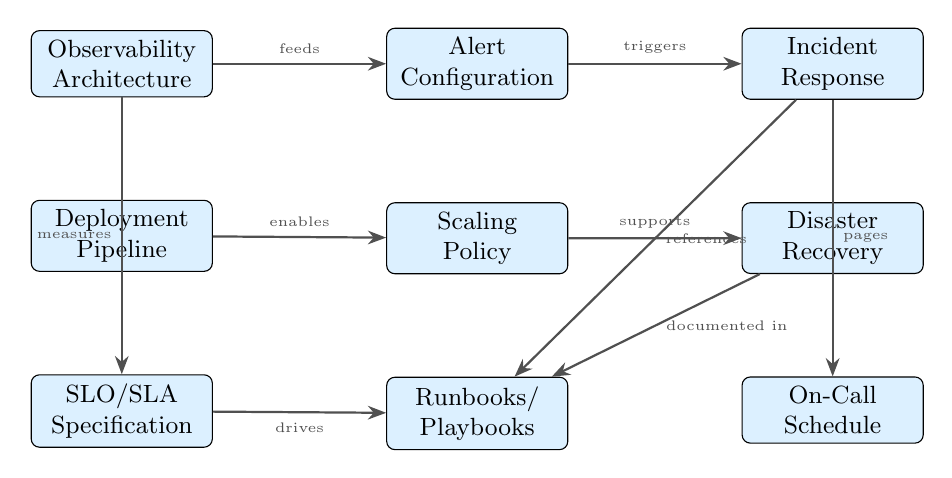
\begin{tikzpicture}[
    node distance=1.3cm and 2cm,
    model/.style={draw, fill=monitorcolor, rounded corners=3pt, minimum width=2.3cm, minimum height=0.75cm, font=\small, align=center},
    arrow/.style={-{Stealth}, thick, darkgray}
]
    % Nodes - top row
    \node[model] (observe) {Observability\\Architecture};
    \node[model, right=2.2cm of observe] (alert) {Alert\\Configuration};
    \node[model, right=2.2cm of alert] (incident) {Incident\\Response};
    
    % Nodes - middle row
    \node[model, below=1.3cm of observe] (deploy) {Deployment\\Pipeline};
    \node[model, below=1.3cm of alert] (scaling) {Scaling\\Policy};
    \node[model, below=1.3cm of incident] (dr) {Disaster\\Recovery};
    
    % Nodes - bottom row
    \node[model, below=1.3cm of deploy] (slo) {SLO/SLA\\Specification};
    \node[model, below=1.3cm of scaling] (runbook) {Runbooks/\\Playbooks};
    \node[model, below=1.3cm of dr] (oncall) {On-Call\\Schedule};
    
    % Arrows
    \draw[arrow] (observe) -- (alert) node[midway, above, font=\tiny] {feeds};
    \draw[arrow] (alert) -- (incident) node[midway, above, font=\tiny] {triggers};
    \draw[arrow] (observe) -- (slo) node[midway, left, font=\tiny] {measures};
    \draw[arrow] (incident) -- (runbook) node[midway, right, font=\tiny] {references};
    \draw[arrow] (incident) -- (oncall) node[midway, right, font=\tiny] {pages};
    \draw[arrow] (deploy) -- (scaling) node[midway, above, font=\tiny] {enables};
    \draw[arrow] (scaling) -- (dr) node[midway, above, font=\tiny] {supports};
    \draw[arrow] (slo) -- (runbook) node[midway, below, font=\tiny] {drives};
    \draw[arrow] (dr) -- (runbook) node[midway, right, font=\tiny] {documented in};
\end{tikzpicture}
\caption{Model Type Dependency Relationships}
\end{figure}

% =============================================================================
% SECTION: MODEL LANGUAGES
% =============================================================================
\section{Model Languages}

For each model type, specific languages, notations, and techniques are prescribed. This section documents the vocabulary for constructing operational views.

\subsection{Observability Diagram Notation}

\begin{figure}[H]
\centering
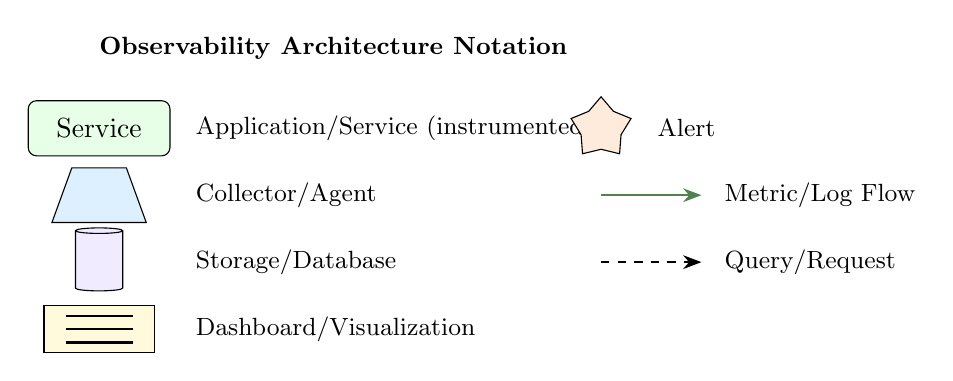
\begin{tikzpicture}[scale=0.85]
    % Legend
    \node[font=\small\bfseries] at (0, 4.5) {Observability Architecture Notation};
    
    % Application/Service
    \node[draw, fill=processcolor, rounded corners=3pt, minimum width=1.8cm, minimum height=0.7cm] at (-3.5, 3.3) {Service};
    \node[right, font=\small] at (-2.2, 3.3) {Application/Service (instrumented)};
    
    % Collector
    \node[draw, fill=monitorcolor, trapezium, trapezium angle=70, minimum width=1.2cm, minimum height=0.5cm] at (-3.5, 2.3) {};
    \node[right, font=\small] at (-2.2, 2.3) {Collector/Agent};
    
    % Storage
    \node[draw, fill=toolcolor, cylinder, shape border rotate=90, aspect=0.3, minimum height=0.8cm, minimum width=0.6cm] at (-3.5, 1.3) {};
    \node[right, font=\small] at (-2.2, 1.3) {Storage/Database};
    
    % Dashboard
    \node[draw, fill=metriccolor, minimum width=1.4cm, minimum height=0.6cm] at (-3.5, 0.3) {};
    \draw[thick] (-4, 0.1) -- (-3, 0.1);
    \draw[thick] (-4, 0.3) -- (-3, 0.3);
    \draw[thick] (-4, 0.5) -- (-3, 0.5);
    \node[right, font=\small] at (-2.2, 0.3) {Dashboard/Visualization};
    
    % Alert
    \node[draw, fill=alertcolor, star, star points=5, minimum size=0.8cm] at (4, 3.3) {};
    \node[right, font=\small] at (4.7, 3.3) {Alert};
    
    % Metric flow
    \draw[-{Stealth}, thick, secondary] (4, 2.3) -- (5.5, 2.3);
    \node[right, font=\small] at (5.7, 2.3) {Metric/Log Flow};
    
    % Query
    \draw[-{Stealth}, thick, dashed] (4, 1.3) -- (5.5, 1.3);
    \node[right, font=\small] at (5.7, 1.3) {Query/Request};
    
\end{tikzpicture}
\caption{Observability Architecture Notation Legend}
\end{figure}

\subsection{Incident Severity Levels}

\begin{table}[H]
\centering
\caption{Standard Incident Severity Classification}
\small
\begin{tabular}{@{}C{1.2cm}L{2.5cm}L{5cm}L{4.5cm}@{}}
\toprule
\textbf{Level} & \textbf{Name} & \textbf{Criteria} & \textbf{Response} \\
\midrule
\cellcolor{critical!30}\textbf{SEV1} & Critical & Complete service outage, data loss risk, security breach & Immediate all-hands, exec notification \\
\addlinespace
\cellcolor{orange!30}\textbf{SEV2} & Major & Significant degradation, major feature unavailable & Immediate on-call response, escalation ready \\
\addlinespace
\cellcolor{warning!30}\textbf{SEV3} & Minor & Limited impact, workaround available & Business hours response, next-day acceptable \\
\addlinespace
\cellcolor{success!30}\textbf{SEV4} & Low & Cosmetic issues, minor inconvenience & Scheduled maintenance window \\
\bottomrule
\end{tabular}
\end{table}

\subsection{SLO Specification Format}

\begin{slobox}[SLO Definition Template]
\begin{tabular}{@{}L{3.5cm}L{10cm}@{}}
\textbf{SLO Name:} & [Descriptive name for the objective] \\
\textbf{Service:} & [Service or system this SLO applies to] \\
\textbf{SLI (Indicator):} & [What is measured - e.g., success rate, latency] \\
\textbf{Target:} & [Numeric target - e.g., 99.9\%, < 200ms p99] \\
\textbf{Window:} & [Measurement window - e.g., rolling 30 days] \\
\textbf{Error Budget:} & [Allowed failures - e.g., 43.2 minutes/month] \\
\textbf{Owner:} & [Team responsible for this SLO] \\
\textbf{Rationale:} & [Business justification for target level] \\
\end{tabular}
\end{slobox}

\subsection{Runbook Structure}

\begin{lstlisting}[caption={Runbook Template Structure}, language={}]
================================================================================
RUNBOOK: [Runbook Title]
================================================================================

METADATA
--------
Runbook ID:     [RB-XXX]
Last Updated:   [Date]
Owner:          [Team/Individual]
Review Date:    [Next review date]
Related Alerts: [Alert names that trigger this runbook]

OVERVIEW
--------
Purpose:        [What this runbook addresses]
Symptoms:       [Observable symptoms that indicate this issue]
Impact:         [Business/user impact of this issue]
Urgency:        [SEV level, response time expectations]

PREREQUISITES
-------------
- Access to [systems/tools required]
- Permissions for [actions needed]
- Knowledge of [relevant background]

DIAGNOSTIC STEPS
----------------
1. [First diagnostic action]
   Expected: [What you should see if this is the issue]
   Command:  [Specific command if applicable]

2. [Second diagnostic action]
   ...

RESOLUTION STEPS
----------------
1. [First resolution action]
   Verification: [How to verify this step succeeded]

2. [Second resolution action]
   ...

ROLLBACK PROCEDURE
------------------
If resolution fails:
1. [Rollback step 1]
2. [Rollback step 2]

ESCALATION
----------
If unresolved after [time]:
- Escalate to: [Team/Individual]
- Contact: [Contact information]
- Provide: [Information needed for escalation]

POST-RESOLUTION
---------------
- [ ] Verify service restored
- [ ] Update incident ticket
- [ ] Notify stakeholders
- [ ] Schedule post-mortem if needed
================================================================================
\end{lstlisting}

\subsection{Deployment Pipeline Notation}

\begin{figure}[H]
\centering
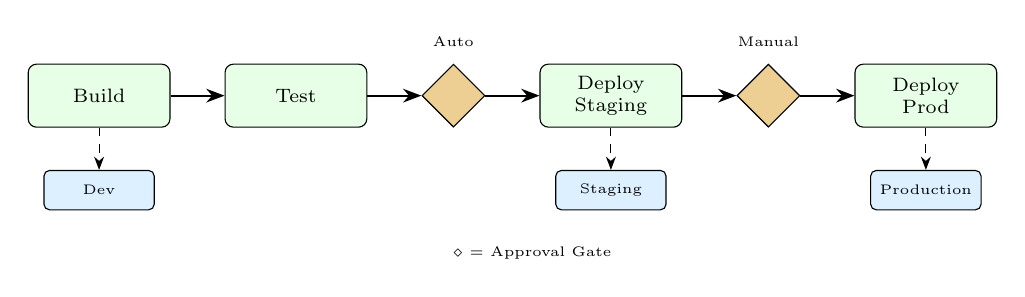
\begin{tikzpicture}[
    stage/.style={draw, fill=processcolor, rounded corners=3pt, minimum width=1.8cm, minimum height=0.8cm, font=\scriptsize, align=center},
    gate/.style={draw, fill=warning!50, diamond, minimum width=0.8cm, minimum height=0.8cm, font=\tiny},
    env/.style={draw, fill=monitorcolor, rounded corners=2pt, minimum width=1.4cm, minimum height=0.5cm, font=\tiny},
]
    % Pipeline stages
    \node[stage] (build) at (0, 0) {Build};
    \node[stage] (test) at (2.5, 0) {Test};
    \node[gate] (gate1) at (4.5, 0) {};
    \node[stage] (staging) at (6.5, 0) {Deploy\\Staging};
    \node[gate] (gate2) at (8.5, 0) {};
    \node[stage] (prod) at (10.5, 0) {Deploy\\Prod};
    
    % Environments
    \node[env] (devenv) at (0, -1.2) {Dev};
    \node[env] (stgenv) at (6.5, -1.2) {Staging};
    \node[env] (prdenv) at (10.5, -1.2) {Production};
    
    % Connections
    \draw[-{Stealth}, thick] (build) -- (test);
    \draw[-{Stealth}, thick] (test) -- (gate1);
    \draw[-{Stealth}, thick] (gate1) -- (staging);
    \draw[-{Stealth}, thick] (staging) -- (gate2);
    \draw[-{Stealth}, thick] (gate2) -- (prod);
    
    \draw[-{Stealth}, dashed] (build) -- (devenv);
    \draw[-{Stealth}, dashed] (staging) -- (stgenv);
    \draw[-{Stealth}, dashed] (prod) -- (prdenv);
    
    % Labels
    \node[font=\tiny, above] at (4.5, 0.5) {Auto};
    \node[font=\tiny, above] at (8.5, 0.5) {Manual};
    
    % Legend
    \node[font=\tiny] at (5.5, -2) {$\diamond$ = Approval Gate};
    
\end{tikzpicture}
\caption{Deployment Pipeline Notation Example}
\end{figure}

\subsection{Tabular Specifications}

\subsubsection{Alert Definition Table}

\begin{table}[H]
\centering
\caption{Example Alert Definition Format}
\small
\begin{tabular}{@{}L{2cm}L{2.5cm}L{2.5cm}L{2cm}L{2cm}L{2cm}@{}}
\toprule
\textbf{Alert} & \textbf{Condition} & \textbf{Threshold} & \textbf{Severity} & \textbf{Team} & \textbf{Runbook} \\
\midrule
HighErrorRate & error\_rate > X & > 1\% for 5m & SEV2 & Platform & RB-001 \\
HighLatency & p99\_latency > X & > 500ms for 10m & SEV3 & Platform & RB-002 \\
DiskSpaceLow & disk\_used > X & > 85\% & SEV3 & Infra & RB-003 \\
ServiceDown & health\_check & failed 3x & SEV1 & On-Call & RB-004 \\
\bottomrule
\end{tabular}
\end{table}

\subsubsection{Backup Schedule Table}

\begin{table}[H]
\centering
\caption{Example Backup Schedule Format}
\small
\begin{tabular}{@{}L{2.2cm}L{2cm}L{2cm}L{2cm}L{2cm}L{2.5cm}@{}}
\toprule
\textbf{System} & \textbf{Type} & \textbf{Frequency} & \textbf{Retention} & \textbf{RPO} & \textbf{Location} \\
\midrule
Primary DB & Full & Daily 2AM & 30 days & 24 hours & S3 us-east-1 \\
Primary DB & Incremental & Hourly & 7 days & 1 hour & S3 us-east-1 \\
User Files & Full & Weekly Sun & 90 days & 7 days & S3 us-west-2 \\
Config Store & Full & Daily & 14 days & 24 hours & S3 us-east-1 \\
\bottomrule
\end{tabular}
\end{table}

% =============================================================================
% SECTION: VIEWPOINT METAMODELS
% =============================================================================
\section{Viewpoint Metamodels}

This section defines the conceptual metamodel underlying the Operational Viewpoint.

\subsection{Core Metamodel}

\begin{figure}[H]
\centering
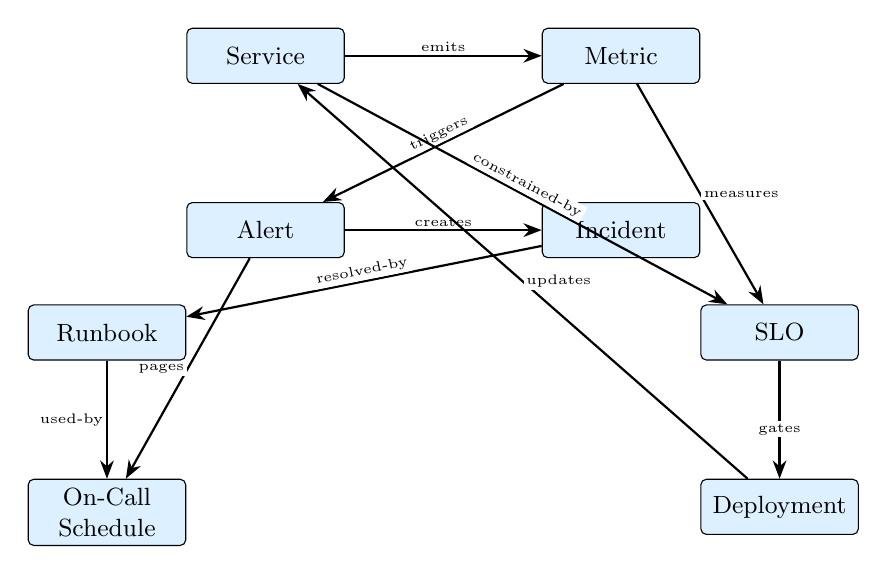
\begin{tikzpicture}[
    node distance=1.3cm and 2cm,
    entity/.style={draw, fill=monitorcolor, rounded corners=2pt, minimum width=2cm, minimum height=0.7cm, font=\small, align=center},
    arrow/.style={-{Stealth}, thick},
    label/.style={font=\tiny, fill=white, inner sep=1pt}
]
    % Main entities
    \node[entity] (service) {Service};
    \node[entity, right=2.5cm of service] (metric) {Metric};
    \node[entity, below=1.5cm of service] (alert) {Alert};
    \node[entity, below=1.5cm of metric] (incident) {Incident};
    \node[entity, below left=2.8cm and 0cm of service] (runbook) {Runbook};
    \node[entity, below right=2.8cm and 0cm of metric] (slo) {SLO};
    \node[entity, below=1.5cm of runbook] (schedule) {On-Call\\Schedule};
    \node[entity, below=1.5cm of slo] (deployment) {Deployment};
    
    % Relationships
    \draw[arrow] (service) -- (metric) node[label, midway, above] {emits};
    \draw[arrow] (metric) -- (alert) node[label, midway, above, sloped] {triggers};
    \draw[arrow] (alert) -- (incident) node[label, midway, above] {creates};
    \draw[arrow] (service) -- (slo) node[label, midway, above, sloped] {constrained-by};
    \draw[arrow] (metric) -- (slo) node[label, midway, right] {measures};
    \draw[arrow] (incident) -- (runbook) node[label, midway, above, sloped] {resolved-by};
    \draw[arrow] (alert) -- (schedule) node[label, midway, left] {pages};
    \draw[arrow] (runbook) -- (schedule) node[label, midway, left] {used-by};
    \draw[arrow] (deployment) -- (service) node[label, midway, right] {updates};
    \draw[arrow] (slo) -- (deployment) node[label, midway, below] {gates};
    
\end{tikzpicture}
\caption{Operational Viewpoint Core Metamodel}
\end{figure}

\subsection{Entity Definitions}

\begin{definitionbox}[Entity: Service]
\textbf{Definition:} An operational unit that provides business functionality and is monitored, deployed, and managed as a cohesive entity.

\textbf{Attributes:}
\begin{itemize}[nosep]
    \item \texttt{serviceId}: Unique identifier
    \item \texttt{name}: Service name
    \item \texttt{description}: Service purpose
    \item \texttt{owner}: Owning team
    \item \texttt{tier}: Criticality tier (Tier 0, 1, 2, 3)
    \item \texttt{dependencies}: Upstream/downstream services
    \item \texttt{healthEndpoint}: Health check URL
    \item \texttt{documentation}: Links to service docs
    \item \texttt{onCallTeam}: Responsible on-call team
    \item \texttt{sloTargets}: Associated SLO references
\end{itemize}

\textbf{Constraints:}
\begin{itemize}[nosep]
    \item Every service must have a defined owner
    \item Tier 0/1 services must have SLOs defined
    \item Services must have health check endpoints
    \item On-call coverage must be assigned
\end{itemize}
\end{definitionbox}

\begin{definitionbox}[Entity: Metric]
\textbf{Definition:} A quantitative measurement collected from a service that indicates its health, performance, or behavior.

\textbf{Attributes:}
\begin{itemize}[nosep]
    \item \texttt{metricId}: Unique identifier
    \item \texttt{name}: Metric name (following naming conventions)
    \item \texttt{type}: Metric type (counter, gauge, histogram, summary)
    \item \texttt{unit}: Unit of measurement
    \item \texttt{labels}: Dimensional labels for filtering
    \item \texttt{source}: Service or component emitting metric
    \item \texttt{frequency}: Collection frequency
    \item \texttt{retention}: How long metric data is retained
    \item \texttt{aggregations}: Supported aggregation methods
\end{itemize}

\textbf{Constraints:}
\begin{itemize}[nosep]
    \item Metric names must follow naming conventions
    \item Label cardinality must be bounded
    \item Critical metrics must have defined retention
\end{itemize}
\end{definitionbox}

\begin{definitionbox}[Entity: Alert]
\textbf{Definition:} A notification triggered when a metric or condition crosses a defined threshold, indicating a potential problem.

\textbf{Attributes:}
\begin{itemize}[nosep]
    \item \texttt{alertId}: Unique identifier
    \item \texttt{name}: Alert name
    \item \texttt{description}: What the alert indicates
    \item \texttt{condition}: Triggering condition/query
    \item \texttt{threshold}: Threshold value(s)
    \item \texttt{duration}: How long condition must persist
    \item \texttt{severity}: Alert severity level
    \item \texttt{recipients}: Teams/individuals to notify
    \item \texttt{channels}: Notification channels (PagerDuty, Slack, email)
    \item \texttt{runbookLink}: Associated runbook
    \item \texttt{suppressionRules}: When to suppress the alert
\end{itemize}

\textbf{Constraints:}
\begin{itemize}[nosep]
    \item Alerts must have associated runbooks
    \item SEV1/2 alerts must page on-call
    \item Alerts should have clear, actionable descriptions
    \item Suppression rules must be documented
\end{itemize}
\end{definitionbox}

\begin{definitionbox}[Entity: Incident]
\textbf{Definition:} An unplanned event that disrupts or degrades service, requiring response and resolution.

\textbf{Attributes:}
\begin{itemize}[nosep]
    \item \texttt{incidentId}: Unique identifier
    \item \texttt{title}: Brief description
    \item \texttt{severity}: Incident severity level
    \item \texttt{status}: Current status (open, investigating, mitigating, resolved)
    \item \texttt{affectedServices}: Services impacted
    \item \texttt{startTime}: When incident began
    \item \texttt{detectionTime}: When incident was detected
    \item \texttt{mitigationTime}: When impact was mitigated
    \item \texttt{resolutionTime}: When fully resolved
    \item \texttt{commander}: Incident commander
    \item \texttt{responders}: Response team members
    \item \texttt{timeline}: Sequence of events and actions
    \item \texttt{rootCause}: Identified root cause
    \item \texttt{actionItems}: Follow-up actions
\end{itemize}

\textbf{Constraints:}
\begin{itemize}[nosep]
    \item SEV1/2 incidents require incident commander
    \item Incidents must have post-mortem within SLA
    \item Timeline must be maintained during incident
    \item Action items must be tracked to completion
\end{itemize}
\end{definitionbox}

\begin{definitionbox}[Entity: SLO (Service Level Objective)]
\textbf{Definition:} A target level of service quality measured by a specific indicator, defining acceptable performance boundaries.

\textbf{Attributes:}
\begin{itemize}[nosep]
    \item \texttt{sloId}: Unique identifier
    \item \texttt{name}: SLO name
    \item \texttt{service}: Associated service
    \item \texttt{sliDefinition}: Service Level Indicator specification
    \item \texttt{target}: Target percentage or value
    \item \texttt{window}: Measurement window (rolling or calendar)
    \item \texttt{errorBudget}: Calculated allowable failures
    \item \texttt{burnRate}: Current consumption rate
    \item \texttt{owner}: Responsible team
    \item \texttt{reviewCadence}: How often SLO is reviewed
\end{itemize}

\textbf{Constraints:}
\begin{itemize}[nosep]
    \item SLO targets must be achievable based on historical data
    \item SLIs must be measurable and automated
    \item Error budgets must have defined policies
    \item SLOs must be reviewed quarterly
\end{itemize}
\end{definitionbox}

\begin{definitionbox}[Entity: Runbook]
\textbf{Definition:} A documented procedure for diagnosing and resolving a specific operational issue or performing a routine task.

\textbf{Attributes:}
\begin{itemize}[nosep]
    \item \texttt{runbookId}: Unique identifier
    \item \texttt{title}: Descriptive title
    \item \texttt{description}: What the runbook addresses
    \item \texttt{triggeringAlerts}: Alerts that reference this runbook
    \item \texttt{prerequisites}: Required access and knowledge
    \item \texttt{diagnosticSteps}: Investigation procedures
    \item \texttt{resolutionSteps}: Fix procedures
    \item \texttt{rollbackSteps}: How to undo changes
    \item \texttt{escalationPath}: When and how to escalate
    \item \texttt{owner}: Maintaining team
    \item \texttt{lastTested}: When last verified
    \item \texttt{lastUpdated}: Last modification date
\end{itemize}

\textbf{Constraints:}
\begin{itemize}[nosep]
    \item Runbooks must be tested at least quarterly
    \item Critical runbooks must have multiple reviewers
    \item Steps must be specific and executable
    \item Runbooks must be kept current with system changes
\end{itemize}
\end{definitionbox}

\begin{definitionbox}[Entity: Deployment]
\textbf{Definition:} A release of software changes to a production environment, including the process, artifacts, and verification.

\textbf{Attributes:}
\begin{itemize}[nosep]
    \item \texttt{deploymentId}: Unique identifier
    \item \texttt{service}: Service being deployed
    \item \texttt{version}: Version being deployed
    \item \texttt{previousVersion}: Version being replaced
    \item \texttt{strategy}: Deployment strategy (rolling, blue-green, canary)
    \item \texttt{artifacts}: Deployed artifacts
    \item \texttt{configChanges}: Configuration changes included
    \item \texttt{deployer}: Person/system initiating deployment
    \item \texttt{approvals}: Required approvals obtained
    \item \texttt{startTime}: Deployment start time
    \item \texttt{endTime}: Deployment completion time
    \item \texttt{status}: Current status (pending, in-progress, completed, rolled-back)
    \item \texttt{verificationResults}: Post-deployment checks
\end{itemize}

\textbf{Constraints:}
\begin{itemize}[nosep]
    \item Production deployments require approval
    \item Deployments must have rollback capability
    \item Verification checks must pass before completion
    \item Deployments must be auditable
\end{itemize}
\end{definitionbox}

\begin{definitionbox}[Entity: On-Call Schedule]
\textbf{Definition:} A rotation defining who is responsible for responding to alerts and incidents during specific time periods.

\textbf{Attributes:}
\begin{itemize}[nosep]
    \item \texttt{scheduleId}: Unique identifier
    \item \texttt{name}: Schedule name
    \item \texttt{team}: Associated team
    \item \texttt{services}: Services covered
    \item \texttt{rotationPeriod}: Length of each rotation (daily, weekly)
    \item \texttt{participants}: Team members in rotation
    \item \texttt{escalationPolicy}: How to escalate if primary unavailable
    \item \texttt{overrides}: Scheduled coverage overrides
    \item \texttt{handoffProcedure}: How shifts are transferred
\end{itemize}

\textbf{Constraints:}
\begin{itemize}[nosep]
    \item 24/7 coverage must be maintained for critical services
    \item Escalation contacts must always be defined
    \item On-call load should be distributed fairly
    \item Handoff procedures must be followed
\end{itemize}
\end{definitionbox}

\subsection{Relationship Definitions}

\begin{table}[H]
\centering
\caption{Metamodel Relationship Definitions}
\small
\begin{tabular}{@{}L{2.3cm}L{1.8cm}L{1.8cm}L{7.5cm}@{}}
\toprule
\textbf{Relationship} & \textbf{Source} & \textbf{Target} & \textbf{Description} \\
\midrule
emits & Service & Metric & Service produces this metric \\
\addlinespace
triggers & Metric & Alert & Metric condition triggers alert \\
\addlinespace
creates & Alert & Incident & Firing alert creates incident \\
\addlinespace
constrained-by & Service & SLO & Service must meet this SLO \\
\addlinespace
measures & Metric & SLO & Metric is used to calculate SLO \\
\addlinespace
resolved-by & Incident & Runbook & Runbook used to resolve incident \\
\addlinespace
pages & Alert & Schedule & Alert notifies on-call via schedule \\
\addlinespace
updates & Deployment & Service & Deployment changes service \\
\addlinespace
gates & SLO & Deployment & SLO status can block deployment \\
\addlinespace
depends-on & Service & Service & Service requires another service \\
\bottomrule
\end{tabular}
\end{table}

% =============================================================================
% SECTION: CONFORMING NOTATIONS
% =============================================================================
\section{Conforming Notations}

Several existing notations and frameworks align with the Operational Viewpoint.

\subsection{ITIL Framework}

ITIL (Information Technology Infrastructure Library) provides comprehensive service management practices that align with operational concerns.

\textbf{Conformance Level:} Framework alignment for service management processes.

\textbf{Key Practices:} Incident Management, Problem Management, Change Management, Service Level Management.

\subsection{SRE Practices}

Google's Site Reliability Engineering practices provide detailed guidance for operational excellence.

\textbf{Conformance Level:} Full alignment for reliability engineering.

\textbf{Key Concepts:} SLOs, Error Budgets, Toil Reduction, Blameless Post-mortems.

\subsection{Prometheus/Grafana Ecosystem}

The Prometheus metrics format and Grafana dashboarding provide de facto standards for observability.

\textbf{Conformance Level:} Tool-specific implementation for monitoring.

\textbf{Key Formats:} PromQL, Grafana JSON dashboard model, Alertmanager configuration.

\subsection{OpenTelemetry}

OpenTelemetry provides vendor-neutral standards for telemetry data.

\textbf{Conformance Level:} Standard for traces, metrics, and logs.

\textbf{Key Specifications:} OTLP protocol, semantic conventions, SDK specifications.

\subsection{Operational Tools Comparison}

\begin{table}[H]
\centering
\caption{Operational Tool Categories}
\small
\begin{tabular}{@{}L{2.8cm}L{4cm}L{6.5cm}@{}}
\toprule
\textbf{Category} & \textbf{Tools} & \textbf{Purpose} \\
\midrule
Metrics & Prometheus, Datadog, New Relic, CloudWatch & Time-series metrics collection and querying \\
\addlinespace
Logging & ELK Stack, Splunk, Loki, CloudWatch Logs & Log aggregation, search, and analysis \\
\addlinespace
Tracing & Jaeger, Zipkin, Datadog APM, X-Ray & Distributed request tracing \\
\addlinespace
Alerting & PagerDuty, OpsGenie, VictorOps & Alert routing and incident management \\
\addlinespace
Dashboarding & Grafana, Datadog, Kibana & Visualization and dashboards \\
\addlinespace
Incident Mgmt & PagerDuty, Jira, ServiceNow & Incident tracking and coordination \\
\addlinespace
On-Call & PagerDuty, OpsGenie, Rootly & On-call scheduling and escalation \\
\addlinespace
Deployment & ArgoCD, Spinnaker, Jenkins, GitHub Actions & CI/CD and deployment automation \\
\bottomrule
\end{tabular}
\end{table}

% =============================================================================
% SECTION: MODEL CORRESPONDENCE RULES
% =============================================================================
\section{Model Correspondence Rules}

Model correspondence rules define how elements in operational models relate to elements in other architectural views.

\subsection{Deployment View Correspondence}

\begin{definitionbox}[Correspondence Rule CR-01: Service to Deployment Mapping]
\textbf{Rule:} Every operational service must correspond to deployed artifacts in the deployment view.

\textbf{Formal Expression:}
\begin{center}
$\forall s \in Services_{Ops} : \exists a \in Artifacts_{Deploy} : implements(a, s)$
\end{center}

\textbf{Rationale:} Ensures operational services have physical deployment presence.

\textbf{Verification:} Deployment manifest review.
\end{definitionbox}

\begin{definitionbox}[Correspondence Rule CR-02: Monitoring Coverage]
\textbf{Rule:} Every deployed component must have corresponding observability instrumentation.

\textbf{Formal Expression:}
\begin{center}
$\forall c \in Components_{Deploy} : \exists M \subseteq Metrics : monitors(M, c)$
\end{center}

\textbf{Rationale:} Ensures complete visibility into deployed systems.

\textbf{Verification:} Metric coverage analysis.
\end{definitionbox}

\subsection{Component-and-Connector View Correspondence}

\begin{definitionbox}[Correspondence Rule CR-03: Health Check Alignment]
\textbf{Rule:} Runtime components must have health endpoints that correspond to operational health checks.

\textbf{Formal Expression:}
\begin{center}
$\forall c \in Components_{C\&C} : \exists h \in HealthChecks : validates(h, c)$
\end{center}

\textbf{Rationale:} Ensures runtime health can be assessed operationally.

\textbf{Verification:} Health endpoint testing.
\end{definitionbox}

\subsection{Quality Attribute Correspondence}

\begin{definitionbox}[Correspondence Rule CR-04: SLO to Requirement Mapping]
\textbf{Rule:} Every availability/performance quality requirement must have a corresponding SLO.

\textbf{Formal Expression:}
\begin{center}
$\forall qr \in QualityRequirements : type(qr) \in \{availability, performance\} \Rightarrow \exists slo \in SLOs : tracks(slo, qr)$
\end{center}

\textbf{Rationale:} Ensures quality requirements are operationally measurable.

\textbf{Verification:} Requirements-to-SLO traceability.
\end{definitionbox}

% =============================================================================
% SECTION: OPERATIONS ON VIEWS
% =============================================================================
\section{Operations on Views}

This section defines the methods for creating, interpreting, analyzing, and implementing operational views.

\subsection{Creation Methods}

\subsubsection{View Development Process}

\begin{guidancebox}[Step 1: Establish Operational Context]
\begin{enumerate}[nosep]
    \item Identify services and components requiring operational support
    \item Gather availability and reliability requirements
    \item Review existing operational processes and tools
    \item Identify operational stakeholders and responsibilities
    \item Assess current operational maturity level
\end{enumerate}
\end{guidancebox}

\begin{guidancebox}[Step 2: Define Observability Strategy]
\begin{enumerate}[nosep]
    \item Identify key metrics for each service (RED: Rate, Errors, Duration)
    \item Define logging strategy and log levels
    \item Plan distributed tracing implementation
    \item Select observability tooling stack
    \item Define retention policies for telemetry data
\end{enumerate}
\end{guidancebox}

\begin{guidancebox}[Step 3: Establish SLOs]
\begin{enumerate}[nosep]
    \item Define SLIs based on user-facing experience
    \item Set initial SLO targets based on historical performance
    \item Calculate error budgets
    \item Define error budget policies
    \item Establish SLO review cadence
\end{enumerate}
\end{guidancebox}

\begin{guidancebox}[Step 4: Design Alerting Strategy]
\begin{enumerate}[nosep]
    \item Define alert severity levels and criteria
    \item Create alerts based on SLOs (multi-window, multi-burn-rate)
    \item Configure alert routing and escalation
    \item Implement alert suppression for maintenance
    \item Document alert-to-runbook mappings
\end{enumerate}
\end{guidancebox}

\begin{guidancebox}[Step 5: Develop Incident Management Process]
\begin{enumerate}[nosep]
    \item Define incident severity classification
    \item Establish incident response procedures
    \item Configure on-call schedules and escalation
    \item Create incident communication templates
    \item Define post-mortem process
\end{enumerate}
\end{guidancebox}

\begin{guidancebox}[Step 6: Plan Deployment and Recovery]
\begin{enumerate}[nosep]
    \item Design deployment pipeline with appropriate gates
    \item Define rollback procedures
    \item Establish backup and recovery procedures
    \item Plan disaster recovery and business continuity
    \item Document deployment runbooks
\end{enumerate}
\end{guidancebox}

\begin{guidancebox}[Step 7: Create Runbooks]
\begin{enumerate}[nosep]
    \item Identify scenarios requiring runbooks
    \item Document diagnostic and resolution procedures
    \item Include escalation paths
    \item Test and validate runbooks
    \item Establish runbook review cycle
\end{enumerate}
\end{guidancebox}

\subsubsection{Common Patterns}

\begin{patternbox}[Pattern: RED Method Metrics]
\textbf{Context:} Need consistent service-level metrics for request-driven services.

\textbf{Solution:} Instrument every service with Rate, Errors, and Duration metrics.

\textbf{Metrics:}
\begin{itemize}[nosep]
    \item \textbf{Rate:} Requests per second
    \item \textbf{Errors:} Failed requests per second
    \item \textbf{Duration:} Distribution of request latencies
\end{itemize}

\textbf{Use When:} Monitoring microservices, APIs, web applications.
\end{patternbox}

\begin{patternbox}[Pattern: USE Method Metrics]
\textbf{Context:} Need consistent resource-level metrics for infrastructure.

\textbf{Solution:} Monitor Utilization, Saturation, and Errors for each resource.

\textbf{Metrics:}
\begin{itemize}[nosep]
    \item \textbf{Utilization:} Percentage of resource capacity used
    \item \textbf{Saturation:} Degree of queuing/waiting
    \item \textbf{Errors:} Error events for the resource
\end{itemize}

\textbf{Use When:} Monitoring infrastructure, databases, queues.
\end{patternbox}

\begin{patternbox}[Pattern: Multi-Window, Multi-Burn-Rate Alerts]
\textbf{Context:} Need alerts that balance responsiveness with noise reduction.

\textbf{Solution:} Use multiple time windows and burn rates to trigger alerts.

\textbf{Configuration:}
\begin{itemize}[nosep]
    \item Short window (5m) + high burn rate (14x) = Page immediately
    \item Medium window (1h) + medium burn rate (6x) = Page
    \item Long window (6h) + low burn rate (1x) = Ticket
\end{itemize}

\textbf{Use When:} SLO-based alerting for critical services.
\end{patternbox}

\begin{patternbox}[Pattern: Canary Deployment]
\textbf{Context:} Need to reduce risk when deploying changes to production.

\textbf{Solution:} Route small percentage of traffic to new version, monitor, then gradually increase.

\textbf{Process:}
\begin{enumerate}[nosep]
    \item Deploy new version alongside current version
    \item Route 1-5\% of traffic to canary
    \item Monitor error rates and latency
    \item Gradually increase traffic if healthy
    \item Auto-rollback if metrics degrade
\end{enumerate}

\textbf{Use When:} Risk-sensitive deployments, services with high traffic.
\end{patternbox}

\begin{table}[H]
\centering
\caption{Operational Patterns Summary}
\small
\begin{tabular}{@{}L{3cm}L{4.5cm}L{5.5cm}@{}}
\toprule
\textbf{Pattern} & \textbf{Description} & \textbf{Use When} \\
\midrule
RED Metrics & Rate, Errors, Duration for services & Request-driven services \\
\addlinespace
USE Metrics & Utilization, Saturation, Errors & Infrastructure monitoring \\
\addlinespace
Golden Signals & Latency, Traffic, Errors, Saturation & Comprehensive service monitoring \\
\addlinespace
Circuit Breaker & Fail fast when dependency fails & Cascading failure prevention \\
\addlinespace
Bulkhead & Isolate failures to components & Fault isolation \\
\addlinespace
Blue-Green Deploy & Two identical environments & Zero-downtime deployment \\
\addlinespace
Canary Deploy & Gradual traffic shift & Risk-sensitive deployment \\
\addlinespace
Feature Flags & Toggle features without deploy & Progressive rollout \\
\addlinespace
Chaos Engineering & Inject failures deliberately & Resilience validation \\
\bottomrule
\end{tabular}
\end{table}

\subsection{Analysis Methods}

\subsubsection{Availability Analysis}

\begin{definitionbox}[Availability Calculation]
\textbf{Purpose:} Calculate and track service availability.

\textbf{Formula:}
\begin{center}
$Availability = \frac{Total Time - Downtime}{Total Time} \times 100\%$
\end{center}

\textbf{Common Targets:}
\begin{itemize}[nosep]
    \item 99\% = 7.3 hours downtime/month
    \item 99.9\% = 43.8 minutes downtime/month
    \item 99.95\% = 21.9 minutes downtime/month
    \item 99.99\% = 4.38 minutes downtime/month
\end{itemize}
\end{definitionbox}

\subsubsection{Error Budget Analysis}

\begin{definitionbox}[Error Budget Calculation]
\textbf{Purpose:} Track remaining budget for failures/changes.

\textbf{Formula:}
\begin{center}
$Error Budget = (1 - SLO Target) \times Window$

$Budget Remaining = Error Budget - Consumed$

$Burn Rate = \frac{Error Rate}{1 - SLO Target}$
\end{center}

\textbf{Example:} 99.9\% SLO over 30 days
\begin{itemize}[nosep]
    \item Error Budget = 0.1\% × 30 days = 43.2 minutes
    \item If 20 minutes consumed, 23.2 minutes remaining
    \item Burn Rate of 2x means budget exhausted in 15 days
\end{itemize}
\end{definitionbox}

\subsubsection{Incident Metrics Analysis}

\begin{definitionbox}[Key Incident Metrics]
\textbf{Purpose:} Measure incident management effectiveness.

\textbf{Key Metrics:}
\begin{itemize}[nosep]
    \item \textbf{MTTD (Mean Time to Detect):} Time from incident start to detection
    \item \textbf{MTTA (Mean Time to Acknowledge):} Time from alert to acknowledgment
    \item \textbf{MTTM (Mean Time to Mitigate):} Time from start to impact mitigation
    \item \textbf{MTTR (Mean Time to Resolve):} Time from start to full resolution
    \item \textbf{Incident Frequency:} Number of incidents per time period
    \item \textbf{Change Failure Rate:} Percentage of deployments causing incidents
\end{itemize}
\end{definitionbox}

% =============================================================================
% SECTION: EXAMPLES
% =============================================================================
\section{Examples}

\subsection{Example 1: Observability Architecture}

\begin{figure}[H]
\centering
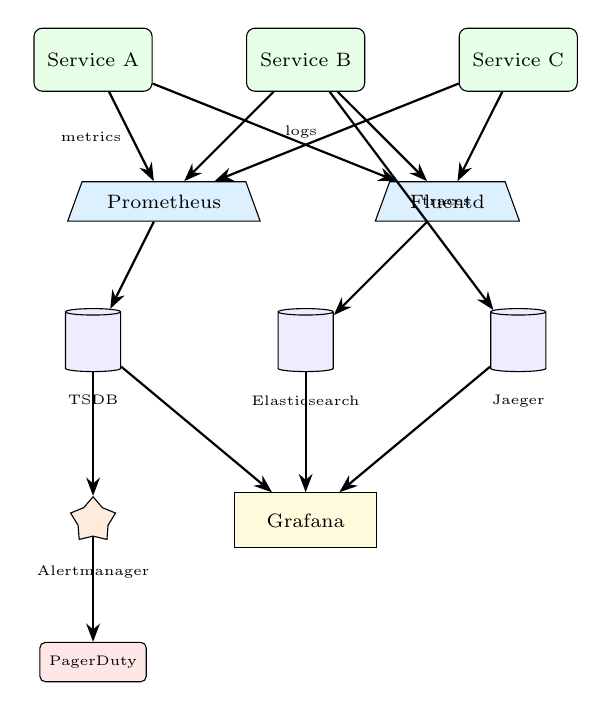
\begin{tikzpicture}[
    service/.style={draw, fill=processcolor, rounded corners=3pt, minimum width=1.5cm, minimum height=0.8cm, font=\scriptsize},
    collector/.style={draw, fill=monitorcolor, trapezium, trapezium angle=70, minimum width=1.2cm, minimum height=0.5cm, font=\scriptsize},
    storage/.style={draw, fill=toolcolor, cylinder, shape border rotate=90, aspect=0.35, minimum height=0.8cm, minimum width=0.7cm, font=\scriptsize},
    dashboard/.style={draw, fill=metriccolor, minimum width=1.8cm, minimum height=0.7cm, font=\scriptsize},
    alert/.style={draw, fill=alertcolor, star, star points=5, minimum size=0.6cm, font=\tiny},
    scale=0.9
]
    % Services
    \node[service] (svc1) at (-3, 3) {Service A};
    \node[service] (svc2) at (0, 3) {Service B};
    \node[service] (svc3) at (3, 3) {Service C};
    
    % Collectors
    \node[collector] (prom) at (-2, 1) {Prometheus};
    \node[collector] (fluentd) at (2, 1) {Fluentd};
    
    % Storage
    \node[storage] (promdb) at (-3, -1) {};
    \node[font=\tiny, below] at (-3, -1.6) {TSDB};
    \node[storage] (elastic) at (0, -1) {};
    \node[font=\tiny, below] at (0, -1.6) {Elasticsearch};
    \node[storage] (jaeger) at (3, -1) {};
    \node[font=\tiny, below] at (3, -1.6) {Jaeger};
    
    % Visualization
    \node[dashboard] (grafana) at (0, -3.5) {Grafana};
    
    % Alerting
    \node[alert] (alertmgr) at (-3, -3.5) {};
    \node[font=\tiny, below] at (-3, -4) {Alertmanager};
    
    % Pager
    \node[draw, fill=incidentcolor, rounded corners=2pt, minimum width=1.2cm, minimum height=0.5cm, font=\tiny] (pager) at (-3, -5.5) {PagerDuty};
    
    % Connections
    \draw[-{Stealth}, thick] (svc1) -- (prom) node[midway, left, font=\tiny] {metrics};
    \draw[-{Stealth}, thick] (svc2) -- (prom);
    \draw[-{Stealth}, thick] (svc3) -- (prom);
    \draw[-{Stealth}, thick] (svc1) -- (fluentd) node[midway, right, font=\tiny] {logs};
    \draw[-{Stealth}, thick] (svc2) -- (fluentd);
    \draw[-{Stealth}, thick] (svc3) -- (fluentd);
    \draw[-{Stealth}, thick] (svc2) -- (jaeger) node[midway, right, font=\tiny] {traces};
    
    \draw[-{Stealth}, thick] (prom) -- (promdb);
    \draw[-{Stealth}, thick] (fluentd) -- (elastic);
    
    \draw[-{Stealth}, thick] (promdb) -- (grafana);
    \draw[-{Stealth}, thick] (elastic) -- (grafana);
    \draw[-{Stealth}, thick] (jaeger) -- (grafana);
    
    \draw[-{Stealth}, thick] (promdb) -- (alertmgr);
    \draw[-{Stealth}, thick] (alertmgr) -- (pager);
    
\end{tikzpicture}
\caption{Observability Architecture Example}
\end{figure}

\subsection{Example 2: Incident Response Process}

\begin{figure}[H]
\centering
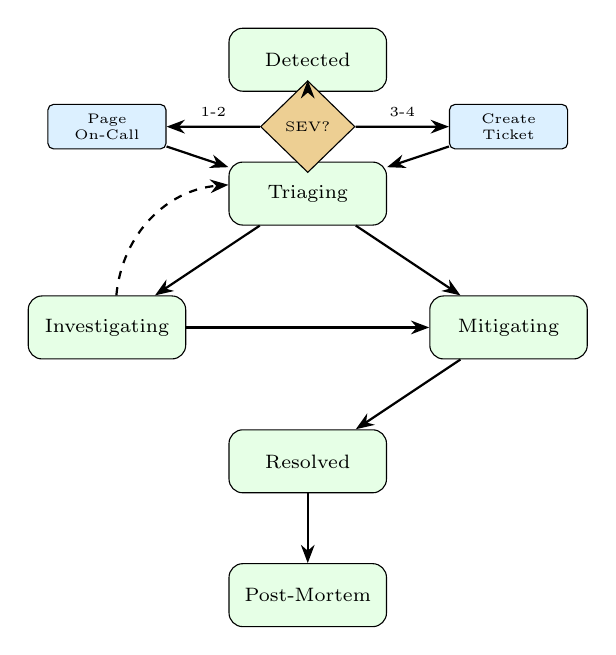
\begin{tikzpicture}[
    state/.style={draw, fill=processcolor, rounded corners=5pt, minimum width=2cm, minimum height=0.8cm, font=\scriptsize},
    decision/.style={draw, fill=warning!50, diamond, minimum width=1.2cm, minimum height=1cm, font=\tiny},
    action/.style={draw, fill=monitorcolor, rounded corners=2pt, minimum width=1.5cm, minimum height=0.5cm, font=\tiny},
    scale=0.85
]
    % States
    \node[state] (detect) at (0, 4) {Detected};
    \node[state] (triage) at (0, 2) {Triaging};
    \node[state] (investigate) at (-3, 0) {Investigating};
    \node[state] (mitigate) at (3, 0) {Mitigating};
    \node[state] (resolved) at (0, -2) {Resolved};
    \node[state] (postmortem) at (0, -4) {Post-Mortem};
    
    % Decision
    \node[decision] (sev) at (0, 3) {SEV?};
    
    % Actions
    \node[action, align=center] (page) at (-3, 3) {Page\\On-Call};
    \node[action, align=center] (ticket) at (3, 3) {Create\\Ticket};
    
    % Connections
    \draw[-{Stealth}, thick] (detect) -- (sev);
    \draw[-{Stealth}, thick] (sev) -- (page) node[midway, above, font=\tiny] {1-2};
    \draw[-{Stealth}, thick] (sev) -- (ticket) node[midway, above, font=\tiny] {3-4};
    \draw[-{Stealth}, thick] (page) -- (triage);
    \draw[-{Stealth}, thick] (ticket) -- (triage);
    \draw[-{Stealth}, thick] (triage) -- (investigate);
    \draw[-{Stealth}, thick] (triage) -- (mitigate);
    \draw[-{Stealth}, thick] (investigate) -- (mitigate);
    \draw[-{Stealth}, thick] (mitigate) -- (resolved);
    \draw[-{Stealth}, thick] (resolved) -- (postmortem);
    
    % Feedback loop
    \draw[-{Stealth}, thick, dashed] (investigate) to[bend left=40] (triage);
    
\end{tikzpicture}
\caption{Incident Response State Machine}
\end{figure}

\subsection{Example 3: SLO Dashboard Specification}

\begin{table}[H]
\centering
\caption{Example SLO Specification}
\small
\begin{tabular}{@{}L{3cm}L{10.5cm}@{}}
\toprule
\multicolumn{2}{l}{\textbf{Service: Payment API}} \\
\midrule
\textbf{SLO Name} & Payment API Availability \\
\textbf{SLI} & Successful requests / Total requests (excluding 4xx) \\
\textbf{Target} & 99.95\% \\
\textbf{Window} & Rolling 30 days \\
\textbf{Error Budget} & 21.9 minutes/month \\
\textbf{Current Status} & 99.97\% (8.7 min consumed, 13.2 min remaining) \\
\textbf{Burn Rate} & 0.4x (healthy) \\
\textbf{Owner} & Payments Team \\
\midrule
\textbf{SLO Name} & Payment API Latency \\
\textbf{SLI} & Requests completing < 500ms / Total requests \\
\textbf{Target} & 99\% \\
\textbf{Window} & Rolling 30 days \\
\textbf{Error Budget} & 7.3 hours/month \\
\textbf{Current Status} & 99.2\% (5.8 hours consumed, 1.5 hours remaining) \\
\textbf{Burn Rate} & 0.8x (caution) \\
\textbf{Owner} & Payments Team \\
\bottomrule
\end{tabular}
\end{table}

% =============================================================================
% SECTION: NOTES
% =============================================================================
\section{Notes}

\subsection{Operational Maturity Model}

\begin{table}[H]
\centering
\caption{Operational Maturity Levels}
\small
\begin{tabular}{@{}C{1.2cm}L{2.5cm}L{5cm}L{4.5cm}@{}}
\toprule
\textbf{Level} & \textbf{Name} & \textbf{Characteristics} & \textbf{Capabilities} \\
\midrule
1 & Reactive & Ad-hoc response, manual processes & Basic monitoring, manual deployment \\
\addlinespace
2 & Defined & Documented processes, some automation & Defined runbooks, CI/CD basics \\
\addlinespace
3 & Measured & SLOs defined, metrics-driven & SLO tracking, automated alerting \\
\addlinespace
4 & Managed & Error budgets, proactive management & Predictive scaling, chaos engineering \\
\addlinespace
5 & Optimized & Continuous improvement, self-healing & Auto-remediation, ML-based ops \\
\bottomrule
\end{tabular}
\end{table}

\subsection{On-Call Best Practices}

\begin{criticalbox}[On-Call Guidelines]
\begin{itemize}[nosep]
    \item Limit on-call shifts to reasonable durations (max 1 week)
    \item Ensure adequate rest between on-call periods
    \item Provide compensation or time-off for on-call duty
    \item Maintain clear escalation paths
    \item Ensure on-call engineers have access to all needed tools
    \item Conduct regular on-call handoffs
    \item Track and reduce on-call burden (toil)
    \item Avoid paging for non-actionable alerts
\end{itemize}
\end{criticalbox}

\subsection{Post-Mortem Best Practices}

\begin{guidancebox}[Blameless Post-Mortem Guidelines]
\begin{itemize}[nosep]
    \item Focus on systems and processes, not individuals
    \item Assume everyone acted with best intentions and available information
    \item Document the complete timeline with evidence
    \item Identify multiple contributing factors
    \item Generate actionable, assigned, and tracked follow-ups
    \item Share learnings broadly across the organization
    \item Review follow-up item completion
    \item Use post-mortems as learning opportunities
\end{itemize}
\end{guidancebox}

\subsection{Common Pitfalls}

\begin{warningbox}[Common Mistakes to Avoid]
\begin{enumerate}[nosep]
    \item \textbf{Alert Fatigue:} Too many alerts leading to ignored pages
    \item \textbf{Missing Runbooks:} Alerts without documented response procedures
    \item \textbf{SLO Without Consequences:} SLOs that don't affect decisions
    \item \textbf{Untested DR:} Disaster recovery plans never validated
    \item \textbf{Manual Toil:} Repetitive tasks not automated
    \item \textbf{Blame Culture:} Post-mortems that assign blame
    \item \textbf{Incomplete Observability:} Blind spots in monitoring coverage
    \item \textbf{Overly Complex Deployments:} Deployments without rollback capability
\end{enumerate}
\end{warningbox}

% =============================================================================
% SECTION: SOURCES
% =============================================================================
\section{Sources}

\subsection{Primary References}

\begin{enumerate}
    \item Beyer, B., Jones, C., Petoff, J., \& Murphy, N. R. (2016). \textit{Site Reliability Engineering: How Google Runs Production Systems}. O'Reilly Media.
    
    \item Beyer, B., Murphy, N. R., Rensin, D. K., Kawahara, K., \& Thorne, S. (2018). \textit{The Site Reliability Workbook}. O'Reilly Media.
    
    \item Kim, G., Humble, J., Debois, P., \& Willis, J. (2016). \textit{The DevOps Handbook}. IT Revolution Press.
    
    \item Limoncelli, T. A., Chalup, S. R., \& Hogan, C. J. (2014). \textit{The Practice of Cloud System Administration}. Addison-Wesley Professional.
    
    \item Majors, C., Fong-Jones, L., \& Miranda, G. (2022). \textit{Observability Engineering}. O'Reilly Media.
\end{enumerate}

\subsection{Supplementary References}

\begin{enumerate}[resume]
    \item Sridharan, C. (2018). \textit{Distributed Systems Observability}. O'Reilly Media.
    
    \item Burns, B. (2018). \textit{Designing Distributed Systems}. O'Reilly Media.
    
    \item Rosenthal, C., \& Jones, N. (2020). \textit{Chaos Engineering}. O'Reilly Media.
    
    \item Forsgren, N., Humble, J., \& Kim, G. (2018). \textit{Accelerate: The Science of Lean Software and DevOps}. IT Revolution Press.
    
    \item AXELOS. (2019). \textit{ITIL Foundation: ITIL 4 Edition}. TSO.
\end{enumerate}

\subsection{Online Resources}

\begin{itemize}
    \item Google SRE Books: \url{https://sre.google/books/}
    \item Prometheus Documentation: \url{https://prometheus.io/docs/}
    \item OpenTelemetry: \url{https://opentelemetry.io/}
    \item PagerDuty Incident Response: \url{https://response.pagerduty.com/}
    \item Grafana Documentation: \url{https://grafana.com/docs/}
\end{itemize}

% =============================================================================
% APPENDIX
% =============================================================================
\appendix

\section{Operational View Checklist}

\begin{table}[H]
\centering
\small
\begin{tabular}{@{}L{10cm}C{2cm}@{}}
\toprule
\textbf{Item} & \textbf{Complete?} \\
\midrule
\multicolumn{2}{l}{\textbf{Observability}} \\
\quad Metrics collection configured for all services & $\square$ \\
\quad Logging aggregation in place & $\square$ \\
\quad Distributed tracing enabled & $\square$ \\
\quad Dashboards created for key services & $\square$ \\
\quad Retention policies defined & $\square$ \\
\midrule
\multicolumn{2}{l}{\textbf{Alerting}} \\
\quad Alert rules defined based on SLOs & $\square$ \\
\quad Alert routing configured & $\square$ \\
\quad Escalation policies in place & $\square$ \\
\quad All alerts linked to runbooks & $\square$ \\
\midrule
\multicolumn{2}{l}{\textbf{Incident Management}} \\
\quad Incident severity levels defined & $\square$ \\
\quad Incident response process documented & $\square$ \\
\quad On-call schedules configured & $\square$ \\
\quad Communication templates ready & $\square$ \\
\quad Post-mortem process defined & $\square$ \\
\midrule
\multicolumn{2}{l}{\textbf{Service Levels}} \\
\quad SLIs defined for critical services & $\square$ \\
\quad SLO targets established & $\square$ \\
\quad Error budgets calculated & $\square$ \\
\quad SLO dashboards created & $\square$ \\
\midrule
\multicolumn{2}{l}{\textbf{Deployment \& Recovery}} \\
\quad Deployment pipeline documented & $\square$ \\
\quad Rollback procedures defined & $\square$ \\
\quad Backup strategy implemented & $\square$ \\
\quad DR plan documented and tested & $\square$ \\
\midrule
\multicolumn{2}{l}{\textbf{Documentation}} \\
\quad Runbooks created for common issues & $\square$ \\
\quad Service catalog maintained & $\square$ \\
\quad Architecture diagrams current & $\square$ \\
\quad On-call documentation complete & $\square$ \\
\bottomrule
\end{tabular}
\end{table}

\section{Glossary}

\begin{description}[style=nextline, leftmargin=3cm, labelwidth=2.8cm]
    \item[Alert] A notification triggered when a monitored condition exceeds a threshold.
    
    \item[Burn Rate] The rate at which error budget is being consumed relative to the SLO window.
    
    \item[Error Budget] The amount of unreliability allowed by an SLO over a given time period.
    
    \item[Incident] An unplanned event causing service disruption or degradation.
    
    \item[Mean Time to Detect (MTTD)] Average time from incident start to detection.
    
    \item[Mean Time to Resolve (MTTR)] Average time from incident start to full resolution.
    
    \item[Observability] The ability to understand system state from external outputs (metrics, logs, traces).
    
    \item[On-Call] A rotation of engineers responsible for responding to production issues.
    
    \item[Post-Mortem] A review conducted after an incident to identify causes and improvements.
    
    \item[Recovery Point Objective (RPO)] Maximum acceptable data loss measured in time.
    
    \item[Recovery Time Objective (RTO)] Maximum acceptable time to restore service after failure.
    
    \item[Runbook] A documented procedure for handling operational tasks or incidents.
    
    \item[Service Level Agreement (SLA)] A contractual commitment to service quality with consequences.
    
    \item[Service Level Indicator (SLI)] A quantitative measure of service quality.
    
    \item[Service Level Objective (SLO)] A target value for an SLI representing desired service quality.
    
    \item[Toil] Repetitive, manual operational work that scales linearly with service growth.
\end{description}

% =============================================================================
% END DOCUMENT
% =============================================================================

\end{document}
